% 07-xr
\begin{frame}[c]{XR}
\begin{columns}[T,onlytextwidth]
\begin{column}{0.30\textwidth}
\textcolor{unired}{\large\bfseries VR}

\small Virtual Reality
\textcolor{unimint}{\rule{\linewidth}{1.6pt}}

A fully virtual environment
\end{column}
\begin{column}{0.30\textwidth}
\textcolor{unired}{\large\bfseries AR}

\small Augmented Reality
\textcolor{unimint}{\rule{\linewidth}{1.6pt}}

Digital content over the real world
\end{column}
\begin{column}{0.30\textwidth}
\textcolor{unired}{\large\bfseries MR}

\small Mixed Reality
\textcolor{unimint}{\rule{\linewidth}{1.6pt}}

Digital objects integrated into real space
\end{column}
\end{columns}
\vspace{0.3cm}
\begin{columns}[c,onlytextwidth]
\begin{column}{0.36\textwidth}
\large This museum uses VR

\vspace{0.15cm}
\small Controllers or hand tracking
\end{column}
\begin{column}{0.28\textwidth}
\centering
\begin{tikzpicture}
  \node[inner sep=0,outer sep=0] (artwork) {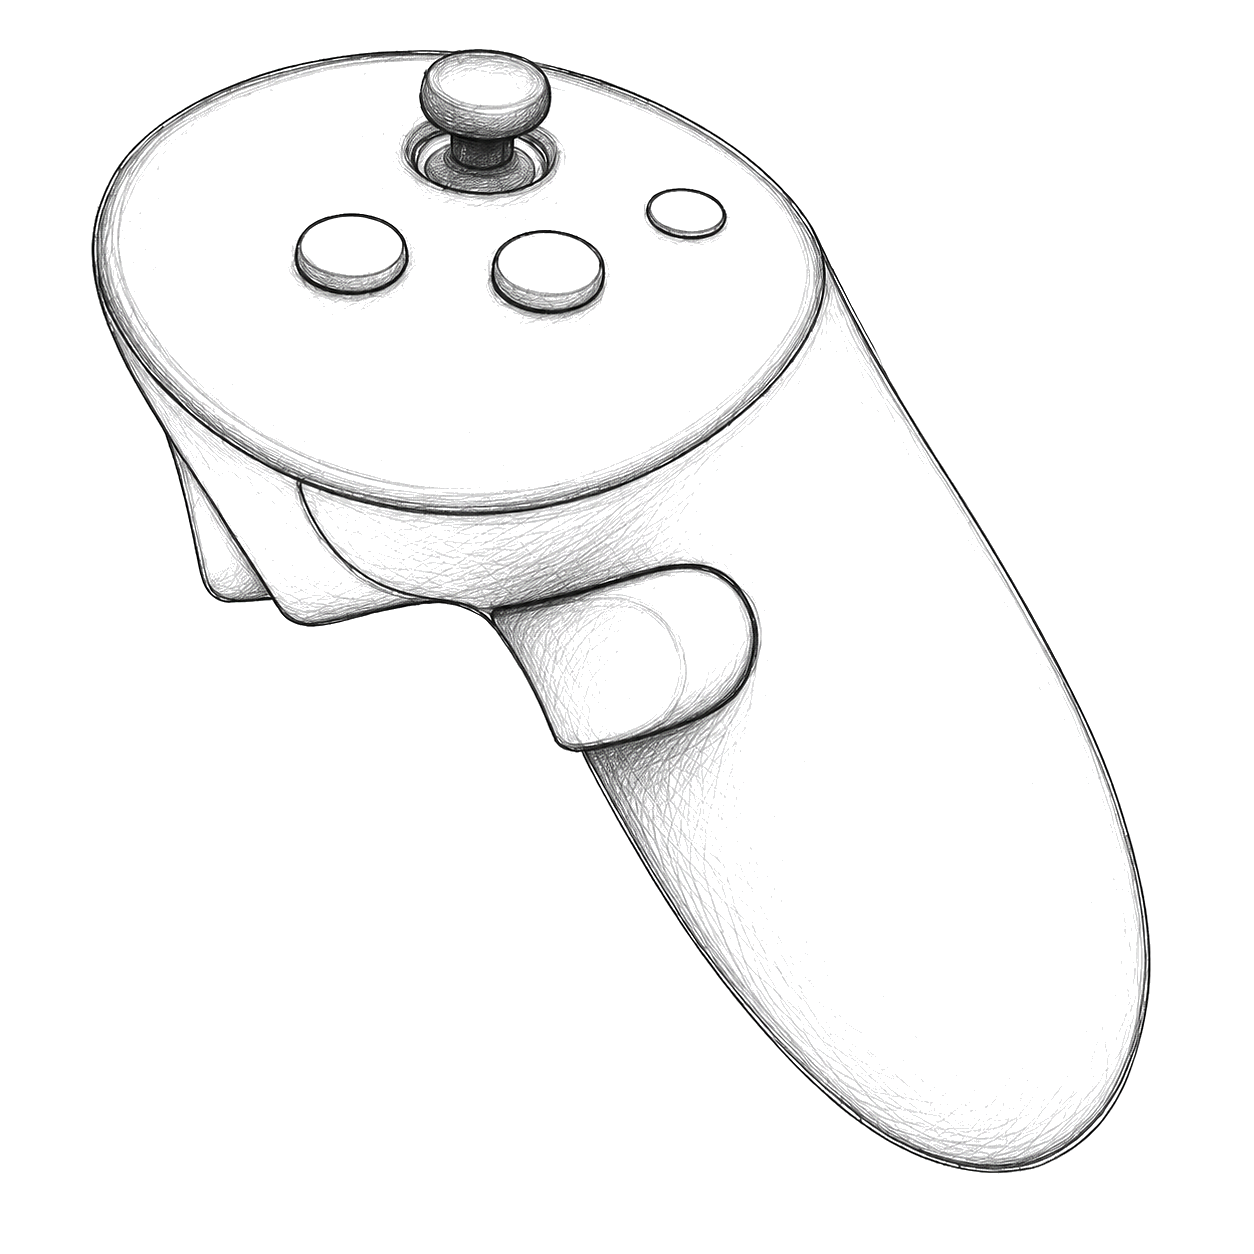
\includegraphics[height=2.05cm,width=\linewidth,keepaspectratio]{Report/Figures/ch04-02-interaction-controller.pdf}};
  \node[anchor=south east,inner sep=1pt,text=black!65,font=\fontsize{4}{5}\selectfont]
    at ([xshift=15pt,yshift=1pt]artwork.south east) {[GPT]};
\end{tikzpicture}

\small Controller
\end{column}
\begin{column}{0.28\textwidth}
\centering
\begin{tikzpicture}
  \node[inner sep=0,outer sep=0] (artwork) {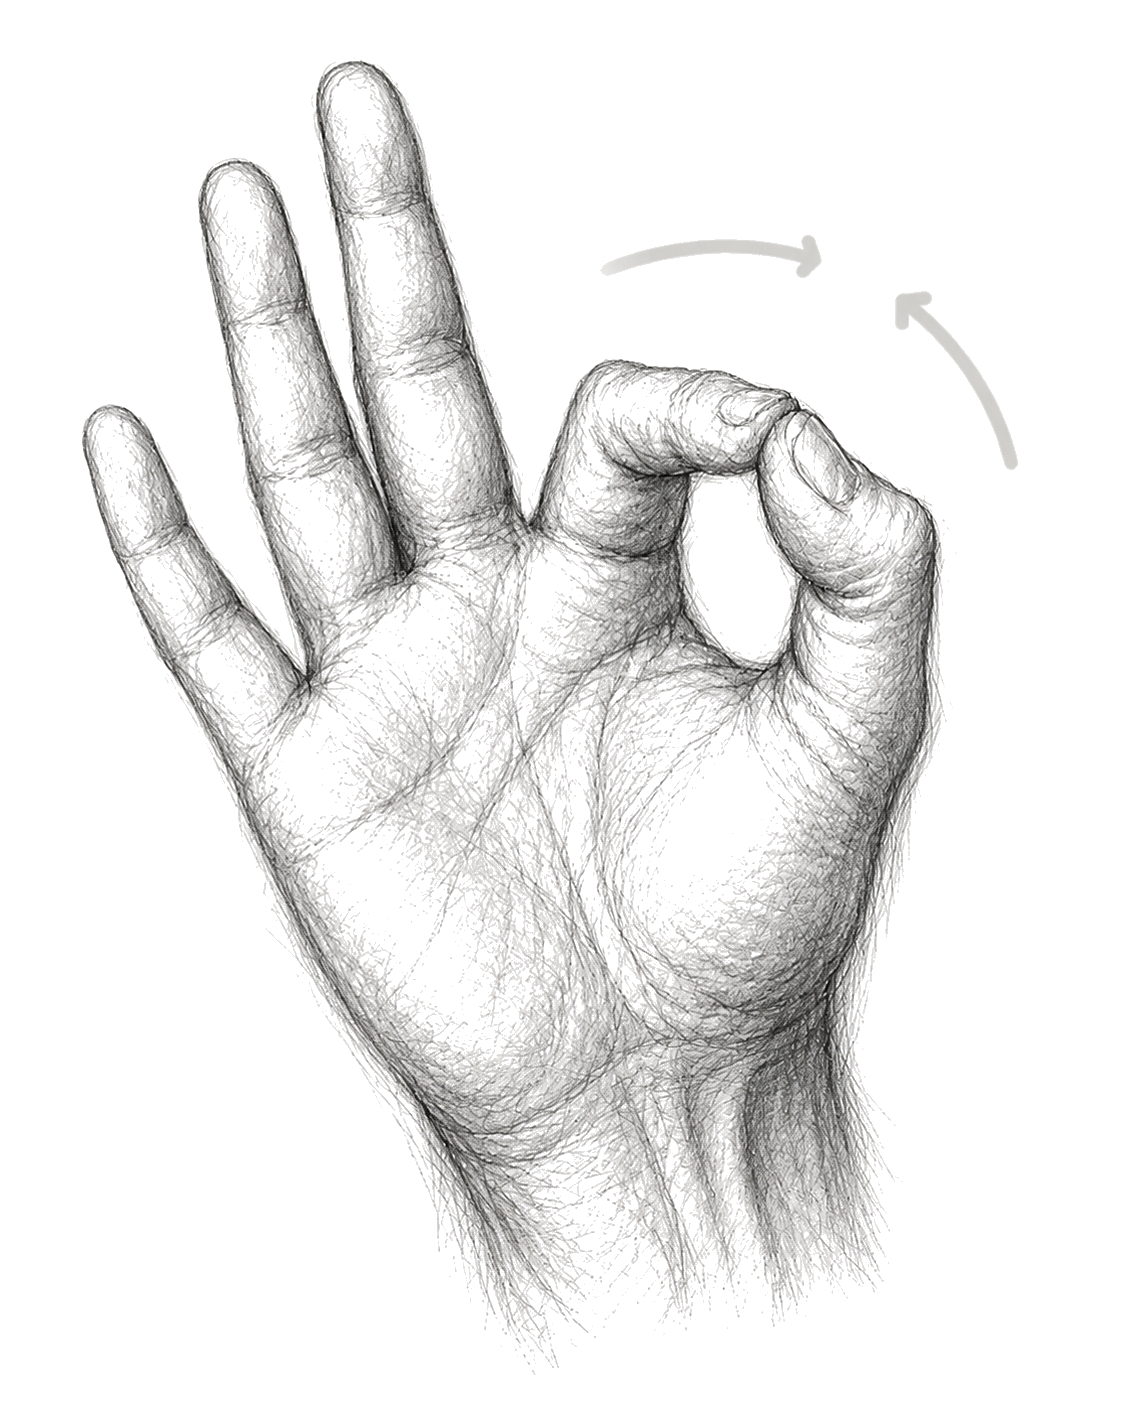
\includegraphics[height=2.05cm,width=\linewidth,keepaspectratio]{Report/Figures/ch04-02-interaction-pinch.pdf}};
  \node[anchor=south east,inner sep=1pt,text=black!65,font=\fontsize{4}{5}\selectfont]
    at ([xshift=15pt,yshift=1pt]artwork.south east) {[GPT]};
\end{tikzpicture}

\small Hand tracking
\end{column}
\end{columns}
\end{frame}
